\chapter{The Prior}

\chapterepigraph
{[T]he problem dealt with is the extrapolation of a very long sequence of symbols\ldots. Almost all, if not all problems in induction can be put in this form.}
{Ray Solomonoff, \textit{A Formal Theory of Inductive Inference} (1964)}

\noindent \textsc{Bayes requires a prior.} If conditioning is the cut the data make, the prior is the cut you make before any data arrive: a decision about how to spread belief over candidates that nothing has yet ruled out. In the classical treatment, it reflects background knowledge, judgment, or convention.

\section*{What kind of measure?}

The Library is generated from strings, but a predictor needs weights, not merely an enumeration. We will build them from a simple experiment: feed fair random bits to a universal computer and ask what output begins to appear. First, though, the weights have to add up to at most $1$.

Start with the most even-handed idea: give every finite string the same weight. It cannot be done. There are infinitely many finite strings, so any fixed positive weight, however small, sums past $1$, and a weight of zero sums to nothing.

The next attempt follows the coin. Flip fair coins and ask how likely the flips are to begin with a given string $s$. The answer is $2^{-|s|}$, where $|s|$ is the length of $s$. Length-$1$ strings each get $1/2$; length-$2$ strings each get $1/4$; and so on. At any fixed length $n$, the $2^n$ strings share the weight exactly: the level sums to $1$.

But the levels are not separate events. Flips that begin with $01$ also begin with $0$; reading $0$ is part of reading $01$. Each level re-counts the same coin flips at a finer grain, so adding the levels counts every run of flips again at every length: $1 + 1 + 1 + \dots$, unbounded. The weights are fine one level at a time. Together they overlap, and the overlap is the whole problem: a stream of bits has no way to say where one string ends.

\section*{Prefix-free codes}

The fix is to remove the overlap: use only a \emph{prefix-free} subset of the strings.

A set of strings is prefix-free if no string in the set is a prefix of another. The set $\{0, 10, 11\}$ is prefix-free. The set $\{0, 01, 11\}$ is not: $0$ is a prefix of $01$.

In the tree of all strings (Figure~\ref{fig:enumeration-tree} from Chapter 2), a prefix-free set corresponds to a collection of nodes whose subtrees are disjoint. Whenever you select a node as a codeword, you cannot also select any of its descendants. The codeword ``claims'' its entire subtree. Figure~\ref{fig:prefix-free-tree} shows an example.

\begin{figure}[h]
\centering
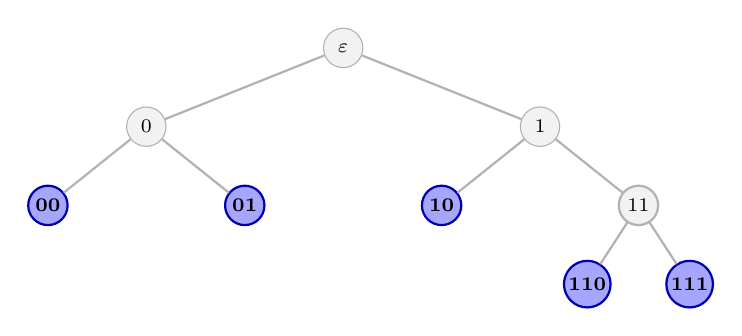
\begin{tikzpicture}[
  level distance=1cm,
  level 1/.style={sibling distance=5cm},
  level 2/.style={sibling distance=2.5cm},
  level 3/.style={sibling distance=1.3cm},
  edge from parent/.style={draw, thick, gray!60}
]
  \node[circle, draw=gray!60, fill=gray!10, inner sep=1pt, minimum size=5mm, font=\scriptsize] {$\varepsilon$}
    child {node[circle, draw=gray!60, fill=gray!10, inner sep=1pt, minimum size=5mm, font=\scriptsize] {0}
      child {node[circle, draw=blue!70!black, fill=blue!35, inner sep=1pt, minimum size=5mm, font=\scriptsize\bfseries] {00}}
      child {node[circle, draw=blue!70!black, fill=blue!35, inner sep=1pt, minimum size=5mm, font=\scriptsize\bfseries] {01}}
    }
    child {node[circle, draw=gray!60, fill=gray!10, inner sep=1pt, minimum size=5mm, font=\scriptsize] {1}
      child {node[circle, draw=blue!70!black, fill=blue!35, inner sep=1pt, minimum size=5mm, font=\scriptsize\bfseries] {10}}
      child {node[circle, draw=gray!60, fill=gray!10, inner sep=1pt, minimum size=5mm, font=\scriptsize] {11}
        child {node[circle, draw=blue!70!black, fill=blue!35, inner sep=1pt, minimum size=5mm, font=\scriptsize\bfseries] {110}}
        child {node[circle, draw=blue!70!black, fill=blue!35, inner sep=1pt, minimum size=5mm, font=\scriptsize\bfseries] {111}}
      }
    };
\end{tikzpicture}
\caption{A prefix-free code as a set of disjoint subtrees. The codewords (filled in blue) are $\{00, 01, 10, 110, 111\}$. Each codeword sits at a node whose entire subtree is ``claimed.'' No codeword is the prefix of another, so the claimed subtrees do not overlap. In this case the codewords also cover the tree: every infinite path passes through exactly one of them.}
\label{fig:prefix-free-tree}
\end{figure}

\section*{Kraft's inequality}

For any prefix-free code with codeword lengths $\ell_1, \ell_2, \ldots$,

$$\sum_i 2^{-\ell_i} \leq 1.$$

This is Kraft's inequality, proved in 1949. The proof is one paragraph.

Consider the unit interval $[0, 1]$. Each codeword $s$ of length $|s|$ corresponds to a sub-interval of width $2^{-|s|}$: the set of real numbers in $[0,1)$ whose binary expansion begins with $s$. The codeword $0$ corresponds to $[0, 1/2)$. The codeword $11$ corresponds to $[3/4, 1)$. The codeword $001$ corresponds to $[1/8, 1/4)$.

If the code is prefix-free, no two of these sub-intervals overlap, because no codeword is a prefix of another. The total width of the sub-intervals is at most $1$, the width of the whole unit interval.

That is Kraft. Prefix-free codes correspond to non-overlapping sub-intervals; non-overlapping sub-intervals fit inside the unit interval; the total widths sum to at most $1$. Figure~\ref{fig:kraft-interval} shows the tiling for the same code.

\begin{figure}[h]
\centering
\begin{tikzpicture}[scale=0.85]
  % Unit interval as a rectangle
  \draw[thick] (0,0) rectangle (12,0.9);
  % Subdivisions for code {00, 01, 10, 110, 111}
  \draw[thick] (3,0) -- (3,0.9);
  \draw[thick] (6,0) -- (6,0.9);
  \draw[thick] (9,0) -- (9,0.9);
  \draw[thick] (10.5,0) -- (10.5,0.9);
  % Codeword labels
  \node[font=\small] at (1.5, 0.45) {$00$};
  \node[font=\small] at (4.5, 0.45) {$01$};
  \node[font=\small] at (7.5, 0.45) {$10$};
  \node[font=\small] at (9.75, 0.45) {$110$};
  \node[font=\small] at (11.25, 0.45) {$111$};
  % Width annotations above
  \draw[<->, thick] (0, 1.2) -- (3, 1.2);
  \node[anchor=south, font=\scriptsize] at (1.5, 1.2) {$2^{-2}$};
  \draw[<->, thick] (9, 1.2) -- (10.5, 1.2);
  \node[anchor=south, font=\scriptsize] at (9.75, 1.2) {$2^{-3}$};
  % Total
  \node[anchor=north, font=\small] at (6, -0.2) {total width $= \tfrac{1}{4} + \tfrac{1}{4} + \tfrac{1}{4} + \tfrac{1}{8} + \tfrac{1}{8} = 1$};
\end{tikzpicture}
\caption{Kraft's inequality as unit-interval tiling. The same prefix-free code $\{00, 01, 10, 110, 111\}$ from Figure~\ref{fig:prefix-free-tree} partitions the unit interval. Each codeword $s$ owns a sub-interval of width $2^{-|s|}$. Because the code is prefix-free, the sub-intervals do not overlap. Their total width is at most $1$. In this case the code is complete and the total is exactly $1$.}
\label{fig:kraft-interval}
\end{figure}

\section*{Fair bits become probability}

Kraft is a fact about prefix-free codes. Fair random bits give it a probabilistic interpretation.

For any prefix-free code, define

$$P(s) = 2^{-|s|}$$

for each codeword $s$. The sum is $\sum_s P(s) = \sum_s 2^{-|s|} \leq 1$ by Kraft. If the sum is less than $1$, treat the missing mass as a residual ``unused'' probability. If the sum equals $1$, the codewords cover everything.

The function $P$ is a subprobability distribution on the codewords: shorter individual codewords carry more weight, with the weights inherited from fair bits on the prefix tree.

Notice exactly what has happened. Kraft makes the length weights $2^{-|s|}$ admissible; it does not make them compulsory. We chose fair bits, and fair bits assign those weights. Other coherent distributions over a prefix-free code are possible. Nor does Kraft say that most of the total mass of an arbitrary code lies on its shortest descriptions: there may be many long codewords.

Finitude supplies a different lesson. A finite reasoner must use bounded representations and local approximations. Short descriptions are useful because they cost less to store and manipulate. That practical pressure does not select a unique prior.

\section*{The universal prior}

Now extend from codewords to programs. Programs are strings; they differ from arbitrary strings only in that they have a runtime behavior on a universal computer.

Let $U$ be a universal machine that reads its program one bit at a time, never going back, and writes its output one symbol at a time, never erasing.\footnote{Machines that read and write this way are called \emph{monotone} machines; Li and Vit\'anyi, \textit{An Introduction to Kolmogorov Complexity and Its Applications}, section~4.5, gives the standard treatment. This form of $M$ is due to Zvonkin and Levin (1970), building on Solomonoff (1964). Machines that must halt are the wrong model here. A halted program has finished its output, so the total weight such programs give to outputs at least $n$ symbols long shrinks toward zero as $n$ grows, and no such sum can keep pace with a source that goes on producing symbols. Halting machines define the exact-output quantity $m_V$ below instead.} Feed it fair coin flips. It need never halt: it reads another bit when it needs one and writes more output when it can. If its output comes to begin with $x$, there is a first moment that happens. Call the bits read up to that moment $p$, a \emph{minimal} program for $x$, and write $U(p) = x{*}$ (Figure~\ref{fig:prefix}). Give each minimal program weight $2^{-|p|}$ and sum:

$$M(x) = \sum_{p \,:\, U(p) = x{*}} 2^{-|p|}.$$

Equivalently, $M(x)$ is the probability that fair coin flips make $U$'s output begin with $x$. The two descriptions give the same number, because each run of flips passes through at most one minimal program for $x$: the bits it had read when $x$ first appeared.

The word \emph{minimal} is doing the work. Because $U$ never erases, once its output begins with $x$ it goes on beginning with $x$ however many further bits it reads. Counting every such extension would re-count the same flips at every length, the overlap from the start of the chapter, and the sum would diverge. Counting only the first moment removes the overlap. (On the output side the overlap is wanted: the weight for $x$ is shared out among its continuations $x0$ and $x1$, and any shortfall is the mass a semimeasure can lose.) No minimal program for $x$ can begin with another one, since the shorter one would have produced $x$ first. So the minimal programs for $x$ form a prefix-free set, and Kraft keeps the sum at most $1$.

\begin{figure}[h]
\centering
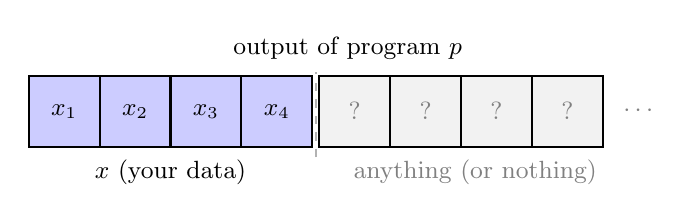
\begin{tikzpicture}[scale=0.9]
  % Prefix x: filled blue boxes
  \foreach \i/\lbl in {0/{$x_1$}, 1/{$x_2$}, 2/{$x_3$}, 3/{$x_4$}} {
    \draw[thick, fill=blue!20] (\i, 0) rectangle ({\i+1}, 1);
    \node[font=\small] at ({\i+0.5}, 0.5) {\lbl};
  }

  % Dashed separator
  \draw[thick, dashed, gray!60] (4.05, -0.15) -- (4.05, 1.05);

  % Continuation: gray "?" boxes
  \foreach \i in {0, 1, 2, 3} {
    \draw[thick, fill=gray!10] ({\i+4.1}, 0) rectangle ({\i+5.1}, 1);
    \node[font=\small, gray] at ({\i+4.6}, 0.5) {$?$};
  }
  \node[font=\small, gray] at (8.6, 0.5) {$\cdots$};

  % Labels below
  \node[anchor=north, font=\small] at (2, -0.05) {$x$ (your data)};
  \node[anchor=north, font=\small, gray] at (6.3, -0.05) {anything (or nothing)};

  % Label above
  \node[anchor=south, font=\small] at (4.5, 1.1) {output of program $p$};
\end{tikzpicture}
\caption{The notation $U(p) = x{*}$ means that $p$ is a minimal program for $x$: when $U$ has read exactly the bits of $p$, its output begins with $x$, and no shorter beginning of $p$ was enough. What follows is any continuation (or none). $M(x)$ sums the weights of all minimal programs for $x$.}
\label{fig:prefix}
\end{figure}

This is Solomonoff's \emph{universal semimeasure} on finite output prefixes $x$.\footnote{It is a semimeasure rather than an ordinary probability measure: probability can be lost when an input produces no further output. Its conditional ratios can still be used for sequential prediction.} It is a distribution for prediction, not yet a measure on realities or on observer occurrences. Figure~\ref{fig:universal-prior} shows $M(x)$ as a cumulative sum over the minimal programs for $x$, ordered by length.

\begin{figure}[h]
\centering
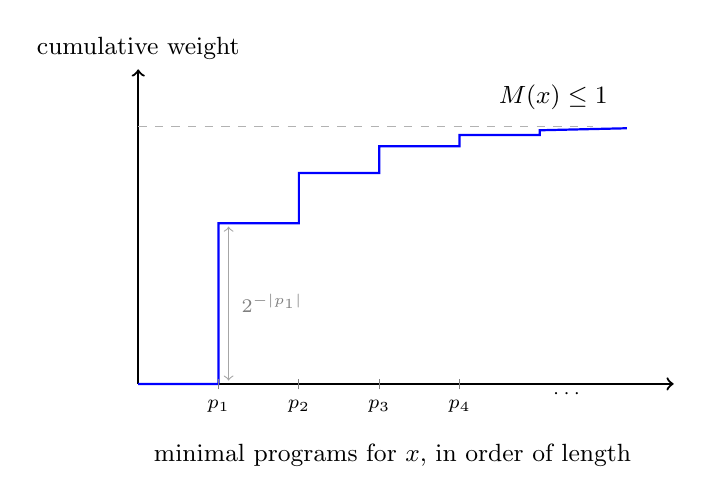
\begin{tikzpicture}[scale=0.85]
  % Axes
  \draw[->, thick] (0, 0) -- (8, 0);
  \draw[->, thick] (0, 0) -- (0, 4.7) node[above, font=\small] {cumulative weight};

  % Asymptote
  \draw[dashed, gray!60] (0, 3.85) -- (6.8, 3.85);

  % Step function (decreasing increments)
  \draw[thick, blue, line cap=square]
    (0, 0) -- (1.2, 0) -- (1.2, 2.4)
    -- (2.4, 2.4) -- (2.4, 3.15)
    -- (3.6, 3.15) -- (3.6, 3.55)
    -- (4.8, 3.55) -- (4.8, 3.72)
    -- (6, 3.72) -- (6, 3.79)
    -- (7.3, 3.82);

  % Tick marks and program labels
  \foreach \x/\p in {1.2/{$p_1$}, 2.4/{$p_2$}, 3.6/{$p_3$}, 4.8/{$p_4$}} {
    \draw[gray] (\x, -0.08) -- (\x, 0.08);
    \node[anchor=north, font=\scriptsize] at (\x, -0.1) {\p};
  }
  \node[font=\scriptsize] at (6.4, -0.15) {$\cdots$};

  % Asymptote label (placed at end of asymptote, inside the plot area)
  \node[anchor=south, font=\small] at (6.2, 3.95) {$M(x) \leq 1$};

  % First step height annotation (inside plot, right of the first step)
  \draw[<->, gray!70, thin] (1.35, 0.05) -- (1.35, 2.35);
  \node[anchor=west, font=\scriptsize, gray] at (1.4, 1.2) {$2^{-|p_1|}$};

  % X-axis caption (below, centered)
  \node[anchor=north, font=\small] at (3.8, -0.75) {minimal programs for $x$, in order of length};
\end{tikzpicture}
\caption{The universal semimeasure $M(x)$ as a cumulative step function. Each minimal program $p$ for $x$ contributes $2^{-|p|}$. Shorter individual programs contribute larger terms. Kraft bounds the completed sum by $1$, because the minimal programs for $x$ form a prefix-free set, but it does not require most of the mass to come from the first few programs.}
\label{fig:universal-prior}
\end{figure}

What $M$ does, in three sentences. It assigns weight to a prefix by summing over every minimal program for it, which comes to the probability that fair coin flips make the machine's output begin with that prefix. A shorter program contributes a larger individual term. Because $U$ is universal, every finite prefix has at least one minimal program, so every prefix gets positive weight.

A related construction connects probability to Kolmogorov complexity, but the distinction matters. Let $V$ be a universal \emph{prefix} machine: its programs must halt, its halting programs form a prefix-free set, and each one ends with an exact finite output. Define

$$m_V(x) = \sum_{q\, :\, V(q)=x} 2^{-|q|}.$$

Let $K_V(x)$ be the length of the shortest program $q$ with $V(q) = x$. Because $V$ is universal, the coding theorem says

$$-\log_2 m_V(x) = K_V(x) + O(1).$$

Thus exact-output algorithmic probability $m_V$ and prefix complexity $K_V$ express the same notion up to an additive constant that depends on $V$. Sequential $M$, by contrast, sums over minimal programs whose output merely begins with the observed data, on a machine that need never halt, and it is the object we condition for prediction. The two constructions are close relatives, not interchangeable notation.

Each program in the sum is a candidate cut: one way of saying what your data are the beginning of. $M$ weights the candidates by the fair-bit experiment, and by nothing else. Whether a heavily weighted description is anything more than a good bet is a question the construction does not ask.

\section*{Where this leaves you}

Bayes needed a prior. Fair coin flips fed to a universal machine that never erases give you one.

The construction is principled but not unique. It depends on a reference universal machine and on the fair-bit distribution. A reasonable agent could write down a different one. Why should this one get special standing?

The next chapter answers with a theorem. $M$ dominates every lower-semicomputable semimeasure up to a constant, and when the data come from a computable source, its predictions converge, with probability one, to the source's own.

That is the optimality.
